\section{Resumen}
En test (relevante = positivo) el Two-Tower supera a EASE en 9 de 9 métricas, promediando 5 semilla(s).

Recall@200: Two-Tower 0.6355 $\pm$ 0.0007, EASE 0.6030, popularidad 0.3332.

Bootstrap de usuarios (semilla 42): la diferencia Two-Tower $-$ EASE es positiva con el IC del 95 \% por encima de 0 en 4 de 4 comparaciones.

Arranque en frío (muestra dev, modelo pequeño de 5 épocas cortas): EASE supera al Two-Tower en 4 de 4 métricas; no es el resultado del conjunto completo y no confirma ventaja en frío.

Watchlist (señal débil, solo dos perfiles) — perfil1: el Two-Tower acierta más que popularidad en el top-50 en 5 de 5 semillas y en el top-200 en 5 de 5; perfil2: el Two-Tower acierta más que popularidad en el top-50 en 0 de 5 semillas y en el top-200 en 5 de 5.

Suite de pruebas: 128 pasadas, 0 saltadas, 0 fallos.

\section{Datos y protocolo}
Recomendador de películas \emph{Two-Tower} entrenado con MovieLens~32M (200\,948 usuarios, 23\,335 películas, 31\,7~M de valoraciones) y
metadatos de TMDB. El reparto es \textbf{por usuario y por tiempo}: el 80\,\% más antiguo de cada usuario es entrenamiento, el 10\,\% siguiente validación y el último 10\,\% test.
Todo lo que se aprende (media de cada usuario, popularidad, vocabularios) sale solo de entrenamiento. En validación el historial de entrada es train; en test, train y validación.
En ambas particiones se excluye del ranking todo lo ya valorado. Las métricas se calculan sobre el catálogo completo (sin muestrear negativos), con una submuestra fija de
20\,000 usuarios elegibles, la misma para los tres métodos. «Relevante» tiene dos definiciones: \emph{positivo} (valoración $\geq \min(4, \bar r_u)$) y valoración $\geq 4$.
Baselines: popularidad (lo más visto en train) y EASE (Steck, 2019, $\lambda=500$) sobre las 10\,000 películas más populares.

\section{Resultados principales}
El Two-Tower se ha entrenado con 5 semilla(s): 42, 43, 44, 45, 46. Cada celda del Two-Tower es la media $\pm$ desviación típica muestral entre semillas; en negrita el mejor método.

\begin{table}[H]\centering\small
\begin{tabular}{lrrr}\toprule
Métrica & Popularidad & EASE & Two-Tower (media $\pm$ desv.) \\\midrule
Recall@10 & 0.0491 & 0.1149 & \textbf{0.1289 $\pm$ 0.0004} \\
Recall@20 & 0.0839 & 0.1897 & \textbf{0.2069 $\pm$ 0.0005} \\
Recall@50 & 0.1495 & 0.3297 & \textbf{0.3526 $\pm$ 0.0006} \\
Recall@200 & 0.3332 & 0.6030 & \textbf{0.6355 $\pm$ 0.0007} \\
NDCG@10 & 0.0497 & 0.1072 & \textbf{0.1231 $\pm$ 0.0003} \\
NDCG@20 & 0.0598 & 0.1292 & \textbf{0.1450 $\pm$ 0.0002} \\
NDCG@50 & 0.0796 & 0.1709 & \textbf{0.1885 $\pm$ 0.0001} \\
NDCG@200 & 0.1273 & 0.2444 & \textbf{0.2644 $\pm$ 0.0002} \\
Cobertura@20 & 0.0144 & 0.1634 & \textbf{0.2043 $\pm$ 0.0027} \\
Novedad@20 & 8.3395 & 10.0466 & \textbf{10.1385 $\pm$ 0.0176} \\
\bottomrule\end{tabular}
\caption{Test, relevante = positivo.}\label{tab:test_pos}
\end{table}

\begin{table}[H]\centering\small
\begin{tabular}{lrrr}\toprule
Métrica & Popularidad & EASE & Two-Tower (media $\pm$ desv.) \\\midrule
Recall@10 & 0.0510 & 0.1178 & \textbf{0.1339 $\pm$ 0.0003} \\
Recall@20 & 0.0868 & 0.1935 & \textbf{0.2133 $\pm$ 0.0004} \\
Recall@50 & 0.1541 & 0.3351 & \textbf{0.3609 $\pm$ 0.0005} \\
Recall@200 & 0.3401 & 0.6080 & \textbf{0.6444 $\pm$ 0.0009} \\
NDCG@10 & 0.0482 & 0.1037 & \textbf{0.1207 $\pm$ 0.0003} \\
NDCG@20 & 0.0589 & 0.1267 & \textbf{0.1441 $\pm$ 0.0002} \\
NDCG@50 & 0.0796 & 0.1692 & \textbf{0.1886 $\pm$ 0.0002} \\
NDCG@200 & 0.1268 & 0.2410 & \textbf{0.2631 $\pm$ 0.0002} \\
Cobertura@20 & 0.0144 & 0.1634 & \textbf{0.2043 $\pm$ 0.0027} \\
Novedad@20 & 8.3395 & 10.0466 & \textbf{10.1385 $\pm$ 0.0176} \\
\bottomrule\end{tabular}
\caption{Test, relevante = valoración $\geq 4$.}\label{tab:test_r4}
\end{table}

\begin{figure}[H]\centering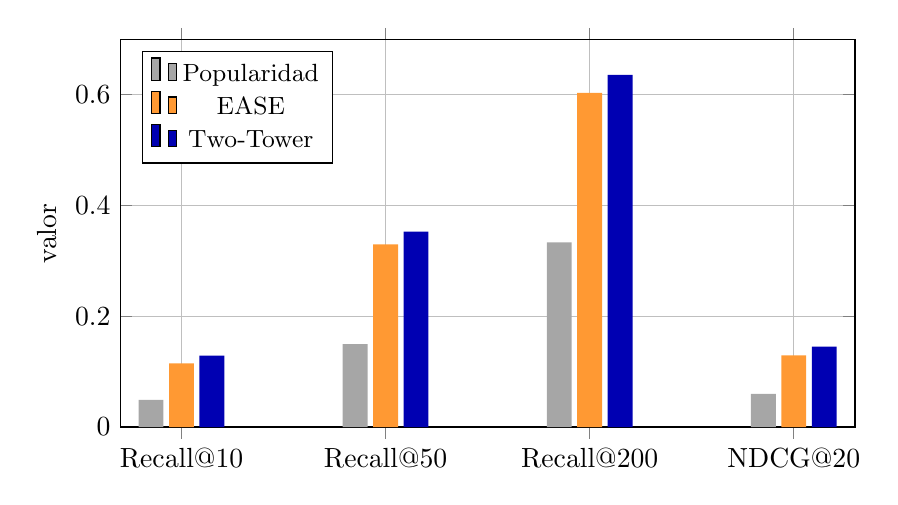
\begin{tikzpicture}\begin{axis}[ybar,width=0.9\linewidth,height=6.5cm,symbolic x coords={Recall@10,Recall@50,Recall@200,NDCG@20},xtick=data,ymin=0,bar width=9pt,legend pos=north west,legend style={font=\small},grid=major,ylabel={valor}]
\addplot[fill=gray!70,draw=none] coordinates {(Recall@10,0.0491) (Recall@50,0.1495) (Recall@200,0.3332) (NDCG@20,0.0598)};\addlegendentry{Popularidad}
\addplot[fill=orange!80,draw=none] coordinates {(Recall@10,0.1149) (Recall@50,0.3297) (Recall@200,0.6030) (NDCG@20,0.1292)};\addlegendentry{EASE}
\addplot[fill=blue!70!black,draw=none] coordinates {(Recall@10,0.1289) (Recall@50,0.3526) (Recall@200,0.6355) (NDCG@20,0.1450)};\addlegendentry{Two-Tower}
\end{axis}\end{tikzpicture}
\caption{Test, relevante = positivo: tres métodos en las métricas principales.}\label{fig:barras}\end{figure}

\begin{table}[H]\centering\small
\begin{tabular}{lrrr}\toprule
Métrica & Popularidad & EASE & Two-Tower (media $\pm$ desv.) \\\midrule
Recall@10 & 0.0548 & 0.1193 & \textbf{0.1373 $\pm$ 0.0009} \\
Recall@20 & 0.0936 & 0.2010 & \textbf{0.2224 $\pm$ 0.0004} \\
Recall@50 & 0.1665 & 0.3539 & \textbf{0.3809 $\pm$ 0.0008} \\
Recall@200 & 0.3561 & 0.6331 & \textbf{0.6709 $\pm$ 0.0004} \\
NDCG@10 & 0.0518 & 0.1066 & \textbf{0.1235 $\pm$ 0.0006} \\
NDCG@20 & 0.0638 & 0.1317 & \textbf{0.1493 $\pm$ 0.0003} \\
NDCG@50 & 0.0862 & 0.1781 & \textbf{0.1977 $\pm$ 0.0004} \\
NDCG@200 & 0.1355 & 0.2540 & \textbf{0.2764 $\pm$ 0.0003} \\
Cobertura@20 & 0.0113 & 0.1597 & \textbf{0.1940 $\pm$ 0.0015} \\
Novedad@20 & 8.3210 & 10.0078 & \textbf{10.0796 $\pm$ 0.0162} \\
\bottomrule\end{tabular}
\caption{Validación, relevante = positivo.}\label{tab:val_pos}
\end{table}

\subsection{Variabilidad entre semillas}
\begin{table}[H]\centering\small
\begin{tabular}{lrrrr}\toprule
Semilla & \texttt{Recall@10} & \texttt{Recall@200} & \texttt{NDCG@20} & \texttt{Cobertura@20} \\\midrule
42 & 0.1291 & 0.6346 & 0.1451 & 0.2041 \\
43 & 0.1283 & 0.6358 & 0.1447 & 0.2012 \\
44 & 0.1294 & 0.6354 & 0.1447 & 0.2087 \\
45 & 0.1289 & 0.6352 & 0.1451 & 0.2043 \\
46 & 0.1290 & 0.6366 & 0.1452 & 0.2033 \\
\bottomrule\end{tabular}
\caption{Two-Tower por semilla en test (relevante = positivo).}\label{tab:semillas}
\end{table}

\subsection{Entrenamiento}
\begin{figure}[H]\centering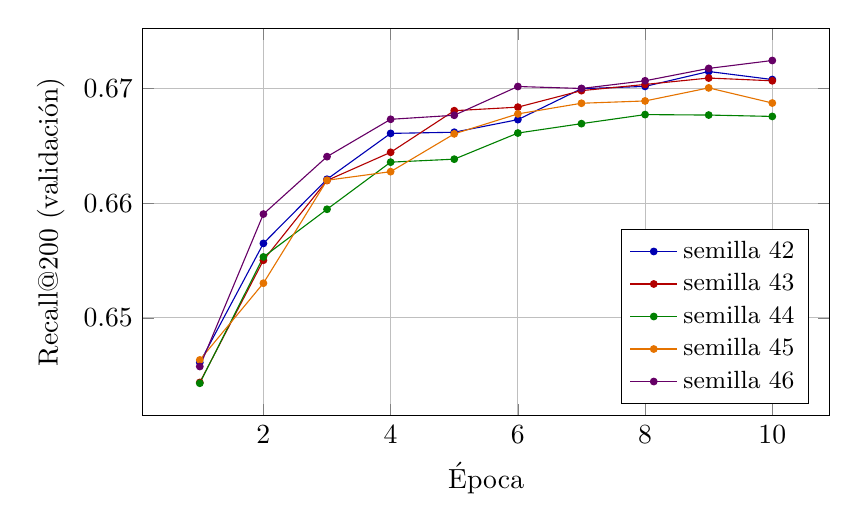
\begin{tikzpicture}\begin{axis}[width=0.85\linewidth,height=6.5cm,xlabel={Época},ylabel={Recall@200 (validación)},grid=both,legend pos=south east,legend style={font=\small}]
\addplot[color=blue!70!black,mark=*,mark size=1.2pt] coordinates {(1,0.6461) (2,0.6565) (3,0.6621) (4,0.6661) (5,0.6662) (6,0.6673) (7,0.67) (8,0.6702) (9,0.6715) (10,0.6708)};
\addlegendentry{semilla 42}
\addplot[color=red!70!black,mark=*,mark size=1.2pt] coordinates {(1,0.64437) (2,0.65503) (3,0.66199) (4,0.66445) (5,0.66808) (6,0.66839) (7,0.66983) (8,0.67037) (9,0.67093) (10,0.67069)};
\addlegendentry{semilla 43}
\addplot[color=green!50!black,mark=*,mark size=1.2pt] coordinates {(1,0.6443) (2,0.65532) (3,0.65948) (4,0.66359) (5,0.66385) (6,0.66613) (7,0.66695) (8,0.66774) (9,0.6677) (10,0.66758)};
\addlegendentry{semilla 44}
\addplot[color=orange!90!black,mark=*,mark size=1.2pt] coordinates {(1,0.64633) (2,0.65303) (3,0.66201) (4,0.66276) (5,0.66606) (6,0.6678) (7,0.66873) (8,0.66893) (9,0.67007) (10,0.66875)};
\addlegendentry{semilla 45}
\addplot[color=violet!80!black,mark=*,mark size=1.2pt] coordinates {(1,0.64576) (2,0.65906) (3,0.66407) (4,0.66733) (5,0.66768) (6,0.67019) (7,0.67002) (8,0.67069) (9,0.67177) (10,0.67246)};
\addlegendentry{semilla 46}
\end{axis}\end{tikzpicture}
\caption{Recall@200 en validación por época, una curva por semilla.}\label{fig:curvas}\end{figure}

\section{Significación estadística}
Bootstrap sobre 20000 usuarios de test (2000 remuestreos, misma lista de usuarios para todos los métodos).
\begin{table}[H]\centering\small
\begin{tabular}{llrcc}\toprule
Comparación & Métrica & Diferencia & IC 95\,\% & ¿Excluye el 0? \\\midrule
Two-Tower $-$ Popularidad & recall@20 & +0.1234 & [+0.1197, +0.1271] & sí \\
Two-Tower $-$ Popularidad & recall@200 & +0.3014 & [+0.2962, +0.3063] & sí \\
Two-Tower $-$ Popularidad & ndcg@20 & +0.0854 & [+0.0830, +0.0879] & sí \\
Two-Tower $-$ Popularidad & ndcg@200 & +0.1370 & [+0.1346, +0.1394] & sí \\
Two-Tower $-$ EASE & recall@20 & +0.0177 & [+0.0149, +0.0204] & sí \\
Two-Tower $-$ EASE & recall@200 & +0.0316 & [+0.0284, +0.0348] & sí \\
Two-Tower $-$ EASE & ndcg@20 & +0.0160 & [+0.0143, +0.0176] & sí \\
Two-Tower $-$ EASE & ndcg@200 & +0.0198 & [+0.0184, +0.0212] & sí \\
\bottomrule\end{tabular}
\caption{Diferencias Two-Tower menos baseline con intervalo de confianza por bootstrap.}\end{table}

\section{Arranque en frío de usuarios}
\begin{table}[H]\centering\small
\begin{tabular}{lrrr}\toprule
Métrica & Popularidad & EASE & Two-Tower \\\midrule
Recall@10 & 0.0446 & 0.0988 & 0.0963 \\
Recall@50 & 0.1517 & 0.3074 & 0.2811 \\
Recall@200 & 0.3370 & 0.5682 & 0.5490 \\
NDCG@20 & 0.0824 & 0.1568 & 0.1487 \\
\bottomrule\end{tabular}
\caption{Arranque en frío (10\,\% de usuarios fuera del entrenamiento; se les da el 80\,\% de su historia y se predice el 20\,\% final). Muestra \texttt{dev}.}\end{table}

\section{Validación con la watchlist}
La watchlist son películas que el usuario marcó como «quiero ver»; el modelo no la usa como entrada. Es una señal débil (intereses, no gustos) y tiende a contener clásicos populares, por eso se compara con popularidad. Se excluyen las ya vistas, y solo se cuentan las emparejadas con el catálogo.
\begin{table}[H]\centering\small
\begin{tabular}{lrrrrr}\toprule
Perfil / semilla & $k$ & Aciertos TT & Aciertos pop. & Lift TT & Lift pop. \\\midrule
perfil1\_s42 & 10 & 9 & 5 & 43.0$\times$ & 23.9$\times$ \\
perfil1\_s42 & 50 & 38 & 24 & 36.3$\times$ & 22.9$\times$ \\
perfil1\_s42 & 200 & 107 & 69 & 25.6$\times$ & 16.5$\times$ \\
perfil1\_s43 & 10 & 9 & 5 & 43.0$\times$ & 23.9$\times$ \\
perfil1\_s43 & 50 & 38 & 24 & 36.3$\times$ & 22.9$\times$ \\
perfil1\_s43 & 200 & 103 & 69 & 24.6$\times$ & 16.5$\times$ \\
perfil1\_s44 & 10 & 9 & 5 & 43.0$\times$ & 23.9$\times$ \\
perfil1\_s44 & 50 & 35 & 24 & 33.4$\times$ & 22.9$\times$ \\
perfil1\_s44 & 200 & 102 & 69 & 24.4$\times$ & 16.5$\times$ \\
perfil1\_s45 & 10 & 9 & 5 & 43.0$\times$ & 23.9$\times$ \\
perfil1\_s45 & 50 & 39 & 24 & 37.3$\times$ & 22.9$\times$ \\
perfil1\_s45 & 200 & 102 & 69 & 24.4$\times$ & 16.5$\times$ \\
perfil1\_s46 & 10 & 9 & 5 & 43.0$\times$ & 23.9$\times$ \\
perfil1\_s46 & 50 & 39 & 24 & 37.3$\times$ & 22.9$\times$ \\
perfil1\_s46 & 200 & 107 & 69 & 25.6$\times$ & 16.5$\times$ \\
perfil2\_s42 & 10 & 0 & 1 & 0.0$\times$ & 27.2$\times$ \\
perfil2\_s42 & 50 & 7 & 9 & 38.1$\times$ & 49.0$\times$ \\
perfil2\_s42 & 200 & 26 & 23 & 35.4$\times$ & 31.3$\times$ \\
perfil2\_s43 & 10 & 0 & 1 & 0.0$\times$ & 27.2$\times$ \\
perfil2\_s43 & 50 & 7 & 9 & 38.1$\times$ & 49.0$\times$ \\
perfil2\_s43 & 200 & 24 & 23 & 32.7$\times$ & 31.3$\times$ \\
perfil2\_s44 & 10 & 1 & 1 & 27.2$\times$ & 27.2$\times$ \\
perfil2\_s44 & 50 & 7 & 9 & 38.1$\times$ & 49.0$\times$ \\
perfil2\_s44 & 200 & 24 & 23 & 32.7$\times$ & 31.3$\times$ \\
perfil2\_s45 & 10 & 1 & 1 & 27.2$\times$ & 27.2$\times$ \\
perfil2\_s45 & 50 & 8 & 9 & 43.6$\times$ & 49.0$\times$ \\
perfil2\_s45 & 200 & 29 & 23 & 39.5$\times$ & 31.3$\times$ \\
perfil2\_s46 & 10 & 0 & 1 & 0.0$\times$ & 27.2$\times$ \\
perfil2\_s46 & 50 & 8 & 9 & 43.6$\times$ & 49.0$\times$ \\
perfil2\_s46 & 200 & 29 & 23 & 39.5$\times$ & 31.3$\times$ \\
\bottomrule\end{tabular}
\caption{Aciertos del top-$k$ en la watchlist del usuario (que el modelo nunca ve). Lift = precisión dividida por la tasa de aciertos del azar.}\end{table}

\section{Comprobaciones y pruebas}

Suite de pruebas automáticas: 128 pasadas, 0 saltadas y 0 fallos. Incluye invariantes sobre las salidas reales del conjunto completo (sin fugas temporales, medias solo de entrenamiento, logQ exacto, historiales sin test).

\begin{table}[H]\centering\small
\begin{tabular}{lccccc}\toprule
Comprobación & s42 & s43 & s44 & s45 & s46 \\\midrule
determinismo & OK & OK & OK & OK & OK \\
exclusion c14 & OK & OK & OK & OK & OK \\
finitud y normas & OK & OK & OK & OK & OK \\
id de peliculas frias & OK & OK & OK & OK & OK \\
invariancia orden historial & OK & OK & OK & OK & OK \\
metricas azar y oraculo & OK & OK & OK & OK & OK \\
numpy igual torch & OK & OK & OK & OK & OK \\
\bottomrule\end{tabular}
\caption{Comprobaciones sobre datos reales, por checkpoint.}\end{table}

\subsection{Latencia de inferencia (CPU, Python)}
Un usuario (torre de usuario, puntuar las 23\,335 películas y top-200 exacto): 1.66~ms. En lotes de 512: 0.247~ms por usuario. Calcular la torre de ítem completa: 60.3~ms (una vez por actualización del modelo).

\section{Limitaciones}
\begin{itemize}
\item EASE se calcula sobre las 10\,000 películas más populares (la inversión densa de las 23\,335 necesita unos 9~GB); con el catálogo completo podría mejorar algo.
\item Las métricas se calculan sobre una submuestra fija de 20\,000 usuarios, no sobre todos los elegibles.
\item El mismo hiperparámetro $\tau=0{,}05$ en todas las semillas: no se ha ajustado por semilla ni se ha barrido en el conjunto completo (solo en \texttt{dev}).
\item La validación con la watchlist y las demos con perfiles de Letterboxd se hacen con dos usuarios: son ilustrativas, no estadísticas.
\end{itemize}
\section{Reproducibilidad}
Código y resultados en el repositorio \texttt{CPIA-recommender}. Entrenamiento: \texttt{python -m src.entrenar --muestra completo --device cuda --tau 0.05 --semilla N}. Evaluación: \texttt{python -m src.evaluar}.
Comprobaciones: \texttt{python -m src.comprobaciones}. Este informe: \texttt{python -m src.informe\_final --compilar}.

\section{Glosario}
Cada métrica, variable y término técnico del informe, tal como se usa en este proyecto. Ordenado por temas.

\subsection*{Datos}
\begin{description}\setlength{\itemsep}{2pt}
\item[MovieLens 32M] Conjunto público de valoraciones de películas (GroupLens): unos 32 millones de valoraciones de 0,5 a 5 estrellas de unos 200 000 usuarios. Es la fuente de las valoraciones.
\item[TMDB] The Movie Database: base de datos pública de películas. Aporta director, reparto, duración, palabras clave y sinopsis, que el modelo usa como «contenido» de cada película.
\item[Letterboxd] Red social de cine. Cada usuario puede exportar sus valoraciones (ratings.csv), películas vistas (watched.csv) y lista de pendientes (watchlist.csv). Se usa para la demo con perfiles reales.
\item[Catálogo] Las 23 335 películas que tienen al menos 20 valoraciones en MovieLens. Son las únicas que el modelo puede recomendar.
\item[user\_idx /\allowbreak{} item\_idx] Números enteros contiguos (0, 1, 2…) que identifican a cada usuario y a cada película dentro del código. Se usan en lugar de los identificadores originales (userId, movieId) porque indexan tablas y matrices.
\item[movieId /\allowbreak{} tmdbId] Identificador de una película en MovieLens /\allowbreak{} en TMDB. El catálogo guarda ambos, y el segundo permite emparejar películas de Letterboxd por la API de TMDB.
\item[Partición (train /\allowbreak{} val /\allowbreak{} test)] Reparto de las valoraciones de cada usuario por orden temporal: el 80 \% más antiguo es train (entrenamiento), el 10 \% siguiente val (validación, para decidir cuándo parar) y el último 10 \% test (evaluación final, que nunca se usa para entrenar ni decidir).
\item[Reparto por usuario y tiempo] Cada usuario se reparte por separado y por fecha, de modo que el modelo nunca aprende de valoraciones posteriores a las que se le piden predecir.
\item[Usuario elegible] Usuario con al menos un positivo en train y al menos una película relevante en la partición que se evalúa. Solo ellos cuentan en las métricas, para no promediar usuarios sin nada que acertar.
\item[Submuestra de 20 000 usuarios] Para ahorrar tiempo, las métricas se calculan con 20 000 usuarios elegibles elegidos al azar con una semilla fija; son los mismos para todos los métodos, de modo que la comparación es justa.
\item[media\_u] Media de las valoraciones de entrenamiento de un usuario. Mide si puntúa alto o bajo en general y sirve para decidir qué le gusta (un 4 es «poco» para quien da muchos 5).
\item[Positivo (relevante «positivo»)] Valoración r $\geq$ min(4, media\_u): lo que se considera que le gusta al usuario. La definición alternativa del informe es «rating $\geq$ 4», un umbral fijo.
\item[Nota baja] Valoración r $\leq$ media\_u $-$ 1 que no es positiva. Se usa como señal de «no le gusta» (bolsa B).
\item[Zona neutra] Valoraciones que no son ni positivas ni notas bajas. Entran en el historial con peso reducido (0,25).
\item[Peso de un ejemplo] Importancia de un positivo de entrenamiento en la pérdida: (1 + max(0, r $-$ media\_u)) $\times$ 0,75 si es de las primeras 24 horas del usuario, sin el 0,75 si no. Premia las valoraciones muy por encima de la media del usuario.
\item[Bolsa A /\allowbreak{} bolsa B] Resumen del historial de un usuario como dos «bolsas» de películas con pesos: la A reúne sus positivos y neutras (lo que le gusta o no le disgusta) y la B sus notas bajas (lo que no le gusta). El orden dentro de la bolsa no importa.
\item[Historial y vista train /\allowbreak{} train\_val] Películas que se le dan al modelo como entrada para describir a un usuario. En validación es solo lo de train; en test, train más validación (vista train\_val), que es lo realista.
\item[Máscara de valorados (C14)] Conjunto de películas que el usuario ya ha valorado. Se excluyen siempre de las recomendaciones al evaluar, y en el entrenamiento se descartan como negativos.
\item[Película fría] Película sin valoraciones en train. El modelo no ha podido aprender su identificador, así que su vector sale solo de su contenido (director, reparto, sinopsis…).
\item[Usuario frío /\allowbreak{} arranque en frío] Usuario que no estaba en el entrenamiento. Se le da una parte de su historia (80 \%) y se mide si el modelo acierta lo que vio después (20 \%). Comprueba que el modelo sirve para gente nueva sin reentrenar.
\item[Watchlist] Lista de películas que un usuario de Letterboxd marcó como «quiero ver». El modelo nunca la usa como entrada; se emplea para una evaluación sin etiquetas.
\item[Emparejado exacto /\allowbreak{} por API] Forma de reconocer una película de Letterboxd en el catálogo: por título y año normalizados (exacto) o, si falla, buscando en TMDB (API). El exacto no une títulos distintos de la misma película.
\end{description}

\subsection*{Modelo}
\begin{description}\setlength{\itemsep}{2pt}
\item[Two-Tower (dos torres)] Arquitectura de recomendación con dos redes: una convierte a cada película en un vector (torre de ítem) y otra a cada usuario en otro vector del mismo espacio (torre de usuario). La afinidad es el producto escalar de ambos.
\item[Vector /\allowbreak{} embedding] Lista de números (aquí 128) que representa a una película o a un usuario. Películas o usuarios parecidos quedan cerca en ese espacio.
\item[d = 128] Dimensión de los vectores de usuario y de película.
\item[Norma L2 /\allowbreak{} similitud coseno] Los vectores se normalizan a longitud 1. Así el producto escalar es el coseno del ángulo entre ellos: 1 si apuntan igual, 0 si son perpendiculares. Es lo que mide cuánto encaja una película con un usuario.
\item[Score] Número que el modelo asigna a un par usuario–película: el producto escalar de sus vectores. Más alto = mejor encaje. Las recomendaciones son las películas de score más alto.
\item[Torre de ítem] Red que combina el contenido de la película (sinopsis, géneros, director, reparto, año, duración) y su identificador, y devuelve su vector.
\item[Torre de usuario] Red que toma la media ponderada de los vectores de las películas de las bolsas A y B del usuario, junto con indicadores (si la bolsa está vacía, cuántas películas) y devuelve su vector.
\item[MiniLM (all-MiniLM-L6-v2)] Modelo de lenguaje ya entrenado y congelado que convierte la sinopsis (más las palabras clave) en un vector de 384 números. No se reentrena.
\item[EmbeddingBag] Capa que convierte una lista de identificadores (los directores o los actores de una película) en la media de sus vectores aprendidos.
\item[Dropout del ID (0,5)] Durante el entrenamiento, en cada paso se anula con probabilidad 0,5 el identificador de cada película. Obliga al modelo a funcionar también solo con el contenido, necesario para películas sin valoraciones.
\item[MLP /\allowbreak{} capa oculta /\allowbreak{} ReLU] MLP (perceptrón multicapa): red de capas lineales con una función no lineal entre ellas. Aquí, dos capas con 256 neuronas ocultas. ReLU: la función que pone a 0 los valores negativos.
\item[Pérdida contrastiva (softmax con negativos del lote)] Función que el entrenamiento minimiza: para cada par usuario–película positivo, sube su score frente al de las demás películas del mismo lote, que actúan como ejemplos negativos.
\item[logQ (corrección del sesgo de muestreo)] Se resta a cada score el logaritmo de la popularidad de la película (log P(i)). Corrige que las películas populares aparecen más como negativos del lote y evita que el modelo aprenda solo popularidad.
\item[Temperatura $\tau$] Parámetro que divide los scores antes del softmax. Con $\tau$ pequeña el modelo se concentra en separar lo mejor; con $\tau$ grande es más permisivo. Aquí $\tau$ = 0,05.
\item[Lote (batch) /\allowbreak{} paso /\allowbreak{} época] Lote: grupo de ejemplos que se procesan a la vez (4 096). Paso: una actualización del modelo con un lote. Época: pasada por todos los ejemplos de entrenamiento (unos 3 700 pasos en el conjunto completo).
\item[AdamW] Algoritmo que ajusta los pesos del modelo para reducir la pérdida; Adam con regularización por decaimiento de pesos (weight decay $10^{-4}$).
\item[Tasa de aprendizaje (lr), calentamiento y decaimiento coseno] lr: cuánto se mueven los pesos en cada paso ($10^{-3}$ como máximo). Calentamiento: sube linealmente durante los primeros 200 pasos. Decaimiento coseno: baja suavemente hasta el 5 \% al final.
\item[Parada temprana (paciencia)] Se evalúa en validación al final de cada época y se para si no mejora el Recall@200 durante 3 épocas seguidas. Evita sobreentrenar.
\item[Checkpoint (mejor.pt /\allowbreak{} ultimo.pt)] Archivo con los pesos del modelo y el estado del entrenamiento. mejor.pt es la época con mejor resultado en validación; ultimo.pt permite reanudar si el entrenamiento se corta.
\item[Semilla] Número que fija el azar del entrenamiento (inicialización de pesos y orden de los ejemplos). Cambiar de semilla mide cuánto depende el resultado de la suerte.
\end{description}

\subsection*{Métodos de referencia}
\begin{description}\setlength{\itemsep}{2pt}
\item[Popularidad] Método sin personalización: recomienda a todos los usuarios las películas con más positivos en train, excluyendo las ya valoradas. Es la referencia más básica.
\item[EASE] «Embarrassingly Shallow Autoencoder» (Steck, 2019): modelo lineal sin red neuronal que aprende, con una fórmula cerrada, qué películas suelen valorarse juntas. Muy fuerte para su sencillez. Aquí con $\lambda$ = 500 y sobre las 10 000 películas más populares.
\item[$\lambda$ de EASE] Regularización de EASE: cuanto mayor, más se suaviza lo aprendido. No confundir con $\lambda$ del MMR.
\item[Azar] Recomendar películas al azar entre las no valoradas. Marca el mínimo esperable.
\item[Oráculo] Recomendador imaginario que conoce las respuestas. Su resultado es el techo posible y sirve para comprobar que la métrica está bien calculada.
\end{description}

\subsection*{Métricas}
\begin{description}\setlength{\itemsep}{2pt}
\item[Top-k] Las k películas con mejor score para un usuario, tras excluir las ya valoradas.
\item[Recall@k] De las películas relevantes de un usuario en esa partición, la fracción que aparece en su top-k. Va de 0 a 1; se promedia entre usuarios. Responde a «¿cuánto de lo que le gustaría encuentro?».
\item[NDCG@k] Normalized Discounted Cumulative Gain: premia acertar y que el acierto esté arriba. Cada acierto en la posición p suma 1/\allowbreak{}log\textsubscript{2}(p + 2); se divide por el máximo posible. De 0 a 1.
\item[Techo de recall] Máximo Recall@k alcanzable: media de min(k, nº de relevantes) /\allowbreak{} nº de relevantes. Si un usuario tiene más de k relevantes, ni un modelo perfecto llega a 1.
\item[Cobertura@k] Fracción del catálogo que aparece en el top-k de al menos un usuario evaluado. Cuanto mayor, más variedad global; una cobertura baja indica que se recomiendan siempre las mismas películas.
\item[Novedad@k] Media de $-$log\textsubscript{2} p(i) de las películas recomendadas, con p(i) la popularidad suavizada en train. Valores altos = recomienda películas poco populares.
\item[Aciertos (hits@k), precisión@k, lift] En la watchlist: aciertos = películas del top-k que están en ella; precisión = aciertos /\allowbreak{} k; lift = precisión dividida por la que tendría el azar (fracción de candidatos que están en la watchlist). Un lift de 30$\times$ es 30 veces mejor que el azar.
\item[MMR (relevancia marginal máxima) y $\lambda$] Reordenación que, en cada paso, elige la película con mejor equilibrio entre relevancia y diferencia con lo ya elegido: $\lambda$ $\cdot$ relevancia $-$ (1 $-$ $\lambda$) $\cdot$ similitud máxima. $\lambda$ = 1 mantiene el ranking original; menor $\lambda$ da más variedad. Aquí $\lambda$ = 0,7.
\end{description}

\subsection*{Estadística}
\begin{description}\setlength{\itemsep}{2pt}
\item[Media $\pm$ desviación típica] Media de un resultado entre semillas y su desviación típica muestral (dividida por n $-$ 1). Indica cuánto cambia el resultado al cambiar solo el azar del entrenamiento.
\item[Bootstrap de usuarios] Técnica para medir la incertidumbre: se repite 2 000 veces el cálculo con usuarios remuestreados con reemplazo y se observa cuánto varía la diferencia entre dos métodos.
\item[Intervalo de confianza (IC) del 95 \%] Rango donde cae el 95 \% de los remuestreos del bootstrap. Si el IC de una diferencia no contiene el 0, la diferencia no se explica por qué usuarios entraron en la muestra.
\item[Diferencia pareada] Diferencia calculada usuario a usuario (el mismo usuario con los dos métodos) y luego promediada. Es más precisa que comparar medias sueltas.
\end{description}

\subsection*{Ingeniería}
\begin{description}\setlength{\itemsep}{2pt}
\item[Fuga de datos (leakage)] Error en el que el modelo usa, al entrenar o evaluar, información que no tendría en la práctica (por ejemplo, valoraciones posteriores a la que predice). Las comprobaciones del informe la descartan.
\item[Invariante] Propiedad que debe cumplirse siempre (por ejemplo, «las medias de usuario salen solo de train»). Se comprueba automáticamente sobre los datos reales.
\item[Determinismo] Dos ejecuciones con los mismos datos y el mismo modelo dan exactamente el mismo resultado.
\item[CSR] Formato compacto de matriz dispersa: guarda solo los elementos no nulos y dónde empieza cada fila. Así se guardan los historiales de millones de usuarios.
\item[float32 /\allowbreak{} norma numérica] Números decimales de 32 bits, los que usan el modelo y los ficheros exportados. Dos cálculos equivalentes pueden diferir en el último decimal (~$10^{-6}$).
\item[Latencia] Tiempo de respuesta, en milisegundos (ms): lo que tarda en producir las recomendaciones para un usuario.
\item[Colab /\allowbreak{} GPU T4] Entorno de Google donde se entrenó el modelo. La GPU T4 es la tarjeta gráfica gratuita que lo acelera: una época tarda unos 5,5 minutos.
\item[Coherencia numpy /\allowbreak{} PyTorch] Comprobación de que el vector de usuario calculado con PyTorch y con la reimplementación en numpy (la que usa la exportación a C) coincide hasta ~$10^{-6}$.
\end{description}
